

%-----------------------------------
% Define document and include general packages
%-----------------------------------
% Tabellen- und Abbildungsverzeichnis stehen normalerweise nicht im
% Inhaltsverzeichnis. Gleiches gilt für das Abkürzungsverzeichnis (siehe unten).
% Manche Dozenten bemängeln das. Die Optionen 'listof=totoc,bibliography=totoc'
% geben das Tabellen- und Abbildungsverzeichnis im Inhaltsverzeichnis (toc=Table
% of Content) aus.
% Da es aber verschiedene Regelungen je nach Dozent geben kann, werden hier
% beide Varianten dargestellt.
\documentclass[12pt,oneside,titlepage,listof=totoc,bibliography=totoc]{scrartcl}
%\documentclass[12pt,oneside,titlepage]{scrartcl}

%-----------------------------------
% Dokumentensprache
%-----------------------------------
%\def\FOMEN{}% Auskommentieren um die Dokumentensprache auf englisch zu ändern
\newif\ifde
\newif\ifen

%-----------------------------------
% Meta informationen
%-----------------------------------
% haenno-apa6-slim: Start
% \input{skripte/meta}

%-----------------------------------
% Meta Informationen zur Arbeit
%-----------------------------------

% Autor
\newcommand{\myAutor}{Henning Beier}

% Adresse
\newcommand{\myAdresse}{Hauptstra\ss e 6 \\ \> \> \> 57234 Wilnsdorf}

% Titel der Arbeit
% \newcommand{\myTitel}{Dialogbasierter Zugriff auf eine KI (künstliches, neuronales Netzwerk) über eine Django REST API (Konzeptionierung und Erstellung Prototyp)}
\newcommand{\myTitel}{Dialogbasierter Zugriff auf eine KI über eine Django REST API}

% Betreuer
\newcommand{\myBetreuer}{Daniel Bitzer}

% Lehrveranstaltung
\newcommand{\myLehrveranstaltung}{IT-Infrastruktur}

% Matrikelnummer
\newcommand{\myMatrikelNr}{517370}

% Ort
\newcommand{\myOrt}{Wilnsdorf}

% Datum der Abgabe
\newcommand{\myAbgabeDatum}{\today}

% Semesterzahl
\newcommand{\mySemesterZahl}{7}

% Name der Hochschule
\newcommand{\myHochschulName}{FOM Hochschule für Oekonomie \& Management}

% Standort der Hochschule
\newcommand{\myHochschulStandort}{Siegen}

% Studiengang
\newcommand{\myStudiengang}{Wirtschaftsinformatik}

% Art der Arbeit
\newcommand{\myThesisArt}{Seminararbeit}

% Zu erlangender akademische Grad
\newcommand{\myAkademischerGrad}{Bachelor of Science (B.Sc.)}

% Firma
\newcommand{\myFirma}{Mustermann GmbH}


\ifdefined\FOMEN
%Englisch
\entrue
\usepackage[english]{babel}
\else
%Deutsch
\detrue
\usepackage[ngerman]{babel}
\fi


% haenno-apa6-slim: End

\newcommand{\langde}[1]{%
   \ifde\selectlanguage{ngerman}#1\fi}
\newcommand{\langen}[1]{%
   \ifen\selectlanguage{english}#1\fi}
\usepackage[utf8]{luainputenc}
\langde{\usepackage[babel,german=quotes]{csquotes}}
\langen{\usepackage[babel,english=british]{csquotes}}
\usepackage[T1]{fontenc}
\usepackage{fancyhdr}
\usepackage{underscore} %added for python code
\usepackage{fancybox}
\usepackage[a4paper, left=4cm, right=2cm, top=4cm, bottom=2cm]{geometry}
\usepackage{graphicx}
\usepackage{colortbl}
\usepackage[capposition=top]{floatrow}
\usepackage{array}
\usepackage{float}      %Positionierung von Abb. und Tabellen mit [H] erzwingen
\usepackage{footnote}
% Darstellung der Beschriftung von Tabellen und Abbildungen (Leitfaden S. 44)
% singlelinecheck=false: macht die Caption linksbündig (statt zentriert)
% labelfont auf fett: (Tabelle x.y:, Abbildung: x.y)
% font auf fett: eigentliche Bezeichnung der Abbildung oder Tabelle
% Fettschrift laut Leitfaden 2018 S. 45
\usepackage[singlelinecheck=false, labelfont=bf, font=bf]{caption}
\usepackage{caption}
\usepackage{enumitem}
\usepackage{amssymb}
\usepackage{mathptmx}
%\usepackage{minted} %Kann für schöneres Syntax Highlighting genutzt werden. ACHTUNG: Python muss installiert sein.
\usepackage[scaled=0.9]{helvet} % Behebt, zusammen mit Package courier, pixelige Überschriften. Ist, zusammen mit mathptx, dem times-Package vorzuziehen. Details: https://latex-kurs.de/fragen/schriftarten/Times_New_Roman.html
\usepackage{courier}
\usepackage{amsmath}
\usepackage[table]{xcolor}
\usepackage{marvosym}			% Verwendung von Symbolen, z.B. perfektes Eurozeichen

\renewcommand\familydefault{\sfdefault}
\usepackage{ragged2e}

% Mehrere Fussnoten nacheinander mit Komma separiert
\usepackage[hang,multiple]{footmisc}
\setlength{\footnotemargin}{1em}

% todo Aufgaben als Kommentare verfassen für verschiedene Editoren
\usepackage{todonotes}

% Verhindert, dass nur eine Zeile auf der nächsten Seite steht
\setlength{\marginparwidth}{2cm}
\usepackage[all]{nowidow}

%-----------------------------------
% Farbdefinitionen
%-----------------------------------
\definecolor{darkblack}{rgb}{0,0,0}
\definecolor{dunkelgrau}{rgb}{0.8,0.8,0.8}
\definecolor{hellgrau}{rgb}{0.0,0.7,0.99}
\definecolor{mauve}{rgb}{0.58,0,0.82}
\definecolor{dkgreen}{rgb}{0,0.6,0}

%-----------------------------------
% Pakete für Tabellen
%-----------------------------------
\usepackage{epstopdf}
\usepackage{nicefrac} % Brüche
\usepackage{multirow}
\usepackage{rotating} % vertikal schreiben
\usepackage{mdwlist}
\usepackage{tabularx}% für Breitenangabe

%-----------------------------------
% sauber formatierter Quelltext
%-----------------------------------
\usepackage{listings}
% JavaScript als Sprache definieren:
\lstdefinelanguage{JavaScript}{
	keywords={break, super, case, extends, switch, catch, finally, for, const, function, try, continue, if, typeof, debugger, var, default, in, void, delete, instanceof, while, do, new, with, else, return, yield, enum, let, await},
	keywordstyle=\color{blue}\bfseries,
	ndkeywords={class, export, boolean, throw, implements, import, this, interface, package, private, protected, public, static},
	ndkeywordstyle=\color{darkgray}\bfseries,
	identifierstyle=\color{black},
	sensitive=false,
	comment=[l]{//},
	morecomment=[s]{/*}{*/},
	commentstyle=\color{purple}\ttfamily,
	stringstyle=\color{red}\ttfamily,
	morestring=[b]',
	morestring=[b]"
}


\definecolor{maroon}{cmyk}{0, 0.87, 0.68, 0.32}
\definecolor{halfgray}{gray}{0.55}
\definecolor{ipython_frame}{RGB}{207, 207, 207}
\definecolor{ipython_bg}{RGB}{247, 247, 247}
\definecolor{ipython_red}{RGB}{186, 33, 33}
\definecolor{ipython_green}{RGB}{0, 128, 0}
\definecolor{ipython_cyan}{RGB}{64, 128, 128}
\definecolor{ipython_purple}{RGB}{170, 34, 255}


\lstset{
    breaklines=true,
    extendedchars=true,
    literate=
    {á}{{\'a}}1 {é}{{\'e}}1 {í}{{\'i}}1 {ó}{{\'o}}1 {ú}{{\'u}}1
    {Á}{{\'A}}1 {É}{{\'E}}1 {Í}{{\'I}}1 {Ó}{{\'O}}1 {Ú}{{\'U}}1
    {à}{{\`a}}1 {è}{{\`e}}1 {ì}{{\`i}}1 {ò}{{\`o}}1 {ù}{{\`u}}1
    {À}{{\`A}}1 {È}{{\'E}}1 {Ì}{{\`I}}1 {Ò}{{\`O}}1 {Ù}{{\`U}}1
    {ä}{{\"a}}1 {ë}{{\"e}}1 {ï}{{\"i}}1 {ö}{{\"o}}1 {ü}{{\"u}}1
    {Ä}{{\"A}}1 {Ë}{{\"E}}1 {Ï}{{\"I}}1 {Ö}{{\"O}}1 {Ü}{{\"U}}1
    {â}{{\^a}}1 {ê}{{\^e}}1 {î}{{\^i}}1 {ô}{{\^o}}1 {û}{{\^u}}1
    {Â}{{\^A}}1 {Ê}{{\^E}}1 {Î}{{\^I}}1 {Ô}{{\^O}}1 {Û}{{\^U}}1
    {œ}{{\oe}}1 {Œ}{{\OE}}1 {æ}{{\ae}}1 {Æ}{{\AE}}1 {ß}{{\ss}}1
    {ç}{{\c c}}1 {Ç}{{\c C}}1 {ø}{{\o}}1 {å}{{\r a}}1 {Å}{{\r A}}1
    {€}{{\EUR}}1 {£}{{\pounds}}1
}

\lstdefinelanguage{python}{
    morekeywords={access,and,break,class,continue,def,del,elif,else,except,exec,finally,for,from,global,if,import,in,is,lambda,not,or,pass,print,raise,return,try,while},
    morekeywords=[2]{abs,all,any,basestring,bin,bool,bytearray,callable,chr,classmethod,cmp,compile,complex,delattr,dict,dir,divmod,enumerate,eval,execfile,file,filter,float,format,frozenset,getattr,globals,hasattr,hash,help,hex,id,input,int,isinstance,issubclass,iter,len,list,locals,long,map,max,memoryview,min,next,object,oct,open,ord,pow,property,range,raw_input,reduce,reload,repr,reversed,round,set,setattr,slice,sorted,staticmethod,str,sum,super,tuple,type,unichr,unicode,vars,xrange,zip,apply,buffer,coerce,intern},
    sensitive=true,
    morecomment=[l]\#,
    morestring=[b]',
    morestring=[b]",
    morestring=[s]{'''}{'''},
    morestring=[s]{"""}{"""},
    morestring=[s]{r'}{'},
    morestring=[s]{r"}{"},
    morestring=[s]{r'''}{'''},
    morestring=[s]{r"""}{"""},
    morestring=[s]{u'}{'},
    morestring=[s]{u"}{"},
    morestring=[s]{u'''}{'''},
    morestring=[s]{u"""}{"""},
    % {replace}{replacement}{lenght of replace}
    % *{-}{-}{1} will not replace in comments and so on
    literate=
    {á}{{\'a}}1 {é}{{\'e}}1 {í}{{\'i}}1 {ó}{{\'o}}1 {ú}{{\'u}}1
    {Á}{{\'A}}1 {É}{{\'E}}1 {Í}{{\'I}}1 {Ó}{{\'O}}1 {Ú}{{\'U}}1
    {à}{{\`a}}1 {è}{{\`e}}1 {ì}{{\`i}}1 {ò}{{\`o}}1 {ù}{{\`u}}1
    {À}{{\`A}}1 {È}{{\'E}}1 {Ì}{{\`I}}1 {Ò}{{\`O}}1 {Ù}{{\`U}}1
    {ä}{{\"a}}1 {ë}{{\"e}}1 {ï}{{\"i}}1 {ö}{{\"o}}1 {ü}{{\"u}}1
    {Ä}{{\"A}}1 {Ë}{{\"E}}1 {Ï}{{\"I}}1 {Ö}{{\"O}}1 {Ü}{{\"U}}1
    {â}{{\^a}}1 {ê}{{\^e}}1 {î}{{\^i}}1 {ô}{{\^o}}1 {û}{{\^u}}1
    {Â}{{\^A}}1 {Ê}{{\^E}}1 {Î}{{\^I}}1 {Ô}{{\^O}}1 {Û}{{\^U}}1
    {œ}{{\oe}}1 {Œ}{{\OE}}1 {æ}{{\ae}}1 {Æ}{{\AE}}1 {ß}{{\ss}}1
    {ç}{{\c c}}1 {Ç}{{\c C}}1 {ø}{{\o}}1 {å}{{\r a}}1 {Å}{{\r A}}1
    {€}{{\EUR}}1 {£}{{\pounds}}1
    %
    {^}{{{\color{ipython_purple}\^{}}}}1
    {=}{{{\color{ipython_purple}=}}}1
    %
    {+}{{{\color{ipython_purple}+}}}1
    {*}{{{\color{ipython_purple}$^\ast$}}}1
    {/}{{{\color{ipython_purple}/}}}1
    %
    {+=}{{{+=}}}1
    {-=}{{{-=}}}1
    {*=}{{{$^\ast$=}}}1
    {/=}{{{/=}}}1,
    literate=
    *{-}{{{\color{ipython_purple}-}}}1
     {?}{{{\color{ipython_purple}?}}}1,
    %
    identifierstyle=\color{black}\ttfamily,
    commentstyle=\color{ipython_cyan}\ttfamily,
    stringstyle=\color{ipython_red}\ttfamily,
    keepspaces=true,
    showspaces=false,
    showstringspaces=false,
    rulecolor=\color{ipython_frame},
    frame=lines,
    frameround={t}{t}{t}{t},
    framexleftmargin=6mm,
    numbers=left,
    numberstyle=\tiny\color{halfgray},
    backgroundcolor=\color{ipython_bg},
    % extendedchars=true,
    basicstyle=\scriptsize,
    keywordstyle=\color{ipython_green}\ttfamily,
}


\lstdefinelanguage{json}{
    %basicstyle=\normalfont\ttfamily,
    identifierstyle=\color{black}\ttfamily,
    commentstyle=\color{ipython_cyan}\ttfamily,
    stringstyle=\color{ipython_red}\ttfamily,
    keepspaces=true,
    showspaces=false,
    showstringspaces=false,
    rulecolor=\color{ipython_frame},
    frame=lines,
    frameround={t}{t}{t}{t},
    framexleftmargin=6mm,
    numbers=left,
    numberstyle=\tiny\color{halfgray},
    backgroundcolor=\color{ipython_bg},
    % extendedchars=true,
    basicstyle=\scriptsize,
    keywordstyle=\color{ipython_green}\ttfamily,
    literate=
     *{0}{{{\color{ipython_cyan}0}}}{1}
      {1}{{{\color{ipython_cyan}1}}}{1}
      {2}{{{\color{ipython_cyan}2}}}{1}
      {3}{{{\color{ipython_cyan}3}}}{1}
      {4}{{{\color{ipython_cyan}4}}}{1}
      {5}{{{\color{ipython_cyan}5}}}{1}
      {6}{{{\color{ipython_cyan}6}}}{1}
      {7}{{{\color{ipython_cyan}7}}}{1}
      {8}{{{\color{ipython_cyan}8}}}{1}
      {9}{{{\color{ipython_cyan}9}}}{1}
      {:}{{{\color{ipython_red}{:}}}}{1}
      {,}{{{\color{ipython_red}{,}}}}{1}
      {\{}{{{\color{ipython_purple}{\{}}}}{1}
      {\}}{{{\color{ipython_purple}{\}}}}}{1}
      {[}{{{\color{ipython_purple}{[}}}}{1}
      {]}{{{\color{ipython_purple}{]}}}}{1},
}

\lstdefinelanguage{bash}{
    %basicstyle=\normalfont\ttfamily,
    identifierstyle=\color{black}\ttfamily,
    commentstyle=\color{ipython_cyan}\ttfamily,
    stringstyle=\color{ipython_red}\ttfamily,
    keepspaces=true,
    showspaces=false,
    showstringspaces=false,
    rulecolor=\color{ipython_frame},
    frame=lines,
    frameround={t}{t}{t}{t},
    framexleftmargin=6mm,
    numbers=none,
    numberstyle=\tiny\color{halfgray},
    backgroundcolor=\color{ipython_bg},
    % extendedchars=true,
    basicstyle=\scriptsize,
    keywordstyle=\color{ipython_green}\ttfamily,
    literate=
     *{0}{{{\color{ipython_cyan}0}}}{1}
      {1}{{{\color{ipython_cyan}1}}}{1}
      {2}{{{\color{ipython_cyan}2}}}{1}
      {3}{{{\color{ipython_cyan}3}}}{1}
      {4}{{{\color{ipython_cyan}4}}}{1}
      {5}{{{\color{ipython_cyan}5}}}{1}
      {6}{{{\color{ipython_cyan}6}}}{1}
      {7}{{{\color{ipython_cyan}7}}}{1}
      {8}{{{\color{ipython_cyan}8}}}{1}
      {9}{{{\color{ipython_cyan}9}}}{1}
      {:}{{{\color{ipython_red}{:}}}}{1}
      {,}{{{\color{ipython_red}{,}}}}{1}
      {\{}{{{\color{ipython_purple}{\{}}}}{1}
      {\}}{{{\color{ipython_purple}{\}}}}}{1}
      {[}{{{\color{ipython_purple}{[}}}}{1}
      {]}{{{\color{ipython_purple}{]}}}}{1},
}



% Better inline directory listings
\definecolor{code-gray}{gray}{0.95}
\newcommand{\code}[1]{\colorbox{code-gray}{\texttt{#1}}}

%\lstset{
%	language=JavaScript,
%	numbers=left,
%	numberstyle=\tiny,
%	numbersep=5pt,
%	breaklines=true,
%	showstringspaces=false,
%	frame=l ,
%	xleftmargin=5pt,
%	xrightmargin=5pt,
%	basicstyle=\ttfamily\scriptsize,
%	stepnumber=1,
%	keywordstyle=\color{blue},          % keyword style
 % 	commentstyle=\color{dkgreen},       % comment style
  %	stringstyle=\color{mauve}         % string literal style
%}

%-----------------------------------
%Literaturverzeichnis Einstellungen
%-----------------------------------

% Biblatex

\usepackage{url}
\urlstyle{same}

% haenno-apa6-slim: Start

%%%% Neuer Leitfaden (2018)
%\usepackage[
%backend=biber,
%style=ext-authoryear-ibid, % Auskommentieren und nächste Zeile einkommentieren, falls "Ebd." (ebenda) nicht für sich-wiederholende Fussnoten genutzt werden soll.
%style=ext-authoryear,
%maxcitenames=3,	% mindestens 3 Namen ausgeben bevor et. al. kommt
%maxbibnames=999,
%mergedate=false,
%date=iso,
%seconds=true, %werden nicht verwendet, so werden aber Warnungen unterdrückt.
%urldate=iso,
%innamebeforetitle,
%dashed=false,
%autocite=footnote,
%doi=false,
%useprefix=true, % 'von' im Namen beachten (beim Anzeigen)
%mincrossrefs = 1
%]{biblatex}%iso dateformat für YYYY-MM-DD

%weitere Anpassungen für BibLaTex
% \input{skripte/modsBiblatex2018}

% haenno-apa6-slim: End

% haenno-apa6-slim: Start

%%%% APA START / Biblatex
%% Zitierung und Literaturverzeichnis nach APA6 der LMU
%% ---> Prof. wünscht APA6 nach LMU PDF Besipielen https://gitlab.com/haenno/fom-latex-apa6/-/blob/master/backup/hinweise-zur-apa.pdf
% Teillösungen von hier... 
% https://tex.stackexchange.com/questions/452228/modifying-bibliography-with-biblatex-biber-apa-style-locationpublisherdoi 
% https://texwelt.de/fragen/2686/wie-formatiere-ich-ein-bibtex-literaturverzeichnis-fur-eine-deutschsprachige-ausgabe-nach-den-regeln-der-apa
% https://tex.stackexchange.com/questions/452032/setting-maxcitenames-for-biblatex-apa (credit dahin für Lösung um die anzahl und wiederholungsnennungen, auch an den entdecker DaMiu)
% https://tex.stackexchange.com/questions/526434/edit-biblatex-apa-style  Lösung Punkt hinter OnlineQuellen entf.  nach Tip, DaMiu 

%% Literaturverzeichnis entsprechend abrufen mit:
% -  Internetquellen: (@online) 	Name Herausgeber Seite (analog Autor), 	Erscheinungsjahr, URL, Abrufdatum-URL
% -  Buch:(@book)				 Autoren,			 Erscheinungsjahr, Titel, ggfls. Hinweis auf Auflage/Band, Verlagsort, Verlagsname
% -  Zeitschriftenartikel(@article)   Autoren,			 Erscheinungsjahr, Titel des Artikel, Titel der Zeitschrift, Ausgabe mit Band- ggfls. Heftnummer, Seitenzahl(en)
% -  Weiter auch  möglich:, Herausgeberwerk (@incollection) und  Buchkapitel- oder beitrag(@inbook)
% (ungetestet bisher : Dissertationen (@phdthesis))


\usepackage[
    style           = apa6, 
    uniquelist      = false,    
    maxcitenames    = 6,
    backend         = biber,
	urldate         = short,
	uniquename 		= true,
	language		= ngerman
	]{biblatex} 
		
	%% START Block für Funktion (1. Nennung von 2-6 Autoren: Alle Namen, danach nur noch 1. Name + et.al) 
	\usepackage{lmodern} 
	\makeatletter
	\newcommand{\apamaxcitenames}{6}
	\DeclareNameFormat{labelname}{%
	  \ifthenelse{\value{uniquelist}>1}
		{\numdef\cbx@min{\value{uniquelist}}}
		{\numdef\cbx@min{\value{minnames}}}%
	  \ifboolexpr{test {\ifnumcomp{\value{listcount}}{=}{1}}
				  or test {\ifnumcomp{\value{listtotal}}{=}{2}}}
		{\usebibmacro{labelname:doname}%
		  {\namepartfamily}%
		  {\namepartfamilyi}%
		  {\namepartgiven}%
		  {\namepartgiveni}%
		  {\namepartprefix}%
		  {\namepartprefixi}%
		  {\namepartsuffix}%
		  {\namepartsuffixi}}
		{\ifboolexpr{test {\ifnumcomp{\value{listtotal}}{>}{\apamaxcitenames}}
					 or test {\ifciteseen}}
		 {\ifnumcomp{\value{listcount}}{<}{\cbx@min + 1}
		   {\usebibmacro{labelname:doname}%
			 {\namepartfamily}%
			 {\namepartfamilyi}%
			 {\namepartgiven}%
			 {\namepartgiveni}%
			 {\namepartprefix}%
			 {\namepartprefixi}%
			 {\namepartsuffix}%
			 {\namepartsuffixi}}
		   {}%
		  \ifnumcomp{\value{listcount}}{=}{\cbx@min + 1}
			{\ifnumcomp{\value{listcount}}{<}{\value{listtotal}}
			  {\printdelim{andothersdelim}\bibstring{andothers}}
			  {\usebibmacro{labelname:doname}%
				{\namepartfamily}%
				{\namepartfamilyi}%
				{\namepartgiven}%
				{\namepartgiveni}%
				{\namepartprefix}%
				{\namepartprefixi}%
				{\namepartsuffix}%
				{\namepartsuffixi}}}
			{}%
		  \ifnumcomp{\value{listcount}}{>}{\cbx@min + 1}
		   {\relax}%
		   {}}%
		 {\usebibmacro{labelname:doname}%
		   {\namepartfamily}%
		   {\namepartfamilyi}%
		   {\namepartgiven}%
		   {\namepartgiveni}%
		   {\namepartprefix}%
		   {\namepartprefixi}%
		   {\namepartsuffix}%
		   {\namepartsuffixi}}}}
	\makeatother 
	\DeclareLanguageMapping{ngerman}{ngerman-apa}
	%% ENDE Block für Funktion (1. Nennung von 2-6 Autoren: Alle Namen, danach nur noch 1. Name + et.al)
	
	\DeclareDelimFormat*{finalnamedelim}{\addspace\bibstring{and}\space} % In Parencite von "&" auf "und" ändern
	%\hypersetup{hidelinks}  %Grüne Links auf Literaturverz. unterdrücken.
	\setlength\bibitemsep{1.3ex} % Abstände im Literaturverzeichnis erhöhen
	\setlength\bibnamesep{1.0ex}
	\AtBeginBibliography{\singlespacing} % Zeilenabstand im Literaturverzeichnis ist Einzeilig - siehe Leitfaden S. 14
	\urlstyle{same} %Standard-Font für Link anstelle der "Schreibmaschinenschrift"
	\DeclareFieldFormat[online]{urldate}{[#1\printfield{urldate}].} 	% Anpassung @online + @misc Bibl: Datum in eckigen Klammern ans Ende
	\DeclareFieldFormat[online]{title}{\mkbibemph{#1}} %Anpassung @online + @misc Titel Kursiv	
	\DeclareFieldFormat[online]{url}{\langde{Verfügbar unter}\langen{Available under}\space \url{#1}} 	%Anpassung @online + @misc Text vor URL
	\renewbibmacro*{url+urldate}{\usebibmacro{url}\setunit{\addspace}\usebibmacro{urldate}}  % URL vor Abrufdatum setzen + getrennte Wörter "Verfügbar" und "Unter" entfernen

%%%% APA ENDE

% haenno-apa6-slim: End


%%%%% Alter Leitfaden. Ggf. Einkommentieren und Bereich hierüber auskommentieren
%\usepackage[
%backend=biber,
%style=numeric,
%citestyle=authoryear,
%url=false,
%isbn=false,
%notetype=footonly,
%hyperref=false,
%sortlocale=de]{biblatex}

%weitere Anpassungen für BibLaTex
% \input{skripte/modsBiblatex}

%%%% Ende Alter Leitfaden

%Bib-Datei einbinden
\addbibresource{literatur.bib}

% Zeilenabstand im Literaturverzeichnis ist Einzeilig
% siehe Leitfaden S. 14
\AtBeginBibliography{\singlespacing}

%-----------------------------------
% Silbentrennung
%-----------------------------------
\usepackage{hyphsubst}
\HyphSubstIfExists{ngerman-x-latest}{%
\HyphSubstLet{ngerman}{ngerman-x-latest}}{}

%-----------------------------------
% Pfad fuer Abbildungen
%-----------------------------------
\graphicspath{{./}{./media/}}

%-----------------------------------
% Weitere Ebene einfügen
%-----------------------------------
% haenno-apa6-slim: Start
% \input{skripte/weitereEbene}

\usepackage{titletoc}

\makeatletter

% Setze die Tiefe des Inhaltsverzeichnis auf 4 Ebenen
% Damit erscheinen \paragraph-Sektionen auch im Inhaltsverzeichnis
\setcounter{secnumdepth}{4}
\setcounter{tocdepth}{4}

% Fuege Abstand nach unten wie in einer normalen \section hinzu
% Andernfalls haette \paragraph keinen Zeilenumbruch
% Der Zeilenumbruch koennte mit einer leeren \mbox{} ersetzt werden
% Jedoch klebt dann der Text relativ nah an der Ueberschrift
\renewcommand{\paragraph}{%
  \@startsection{paragraph}{4}%
  {\z@}{3.25ex \@plus 1ex \@minus .2ex}{1.5ex plus 0.2ex}%
  {\normalfont\normalsize\bfseries\sffamily}%
}

\makeatother


% haenno-apa6-slim: End

%-----------------------------------
% Paket für die Nutzung von Anhängen
%-----------------------------------
\usepackage{appendix}

%-----------------------------------
% Zeilenabstand 1,5-zeilig
%-----------------------------------
\usepackage{setspace}
\onehalfspacing

%-----------------------------------
% Absätze durch eine neue Zeile
%-----------------------------------
\setlength{\parindent}{0mm}
\setlength{\parskip}{0.8em plus 0.5em minus 0.3em}

\sloppy					%Abstände variieren
\pagestyle{headings}

%----------------------------------
% Präfix in das Abbildungs- und Tabellenverzeichnis aufnehmen, statt nur der Nummerierung (siehe Issue #206).
%----------------------------------
\KOMAoption{listof}{entryprefix} % Siehe KOMA-Script Doku v3.28 S.153
\BeforeStartingTOC[lof]{\renewcommand*\autodot{:}} % Für den Doppelpunkt hinter Präfix im Abbildungsverzeichnis
\BeforeStartingTOC[lot]{\renewcommand*\autodot{:}} % Für den Doppelpunkt hinter Präfix im Tabellenverzeichnis

%-----------------------------------
% Abkürzungsverzeichnis
%-----------------------------------
\usepackage[printonlyused]{acronym}

%-----------------------------------
% Symbolverzeichnis
%-----------------------------------
% Quelle: https://www.namsu.de/Extra/pakete/Listofsymbols.pdf
% \usepackage[final]{listofsymbols}

%-----------------------------------
% Glossar
%-----------------------------------
\usepackage{glossaries}
\glstoctrue %Auskommentieren, damit das Glossar nicht im Inhaltsverzeichnis angezeigt wird.
\makenoidxglossaries
% haenno-apa6-slim: Start
% \input{abkuerzungen/glossar}

\newglossaryentry{glossar}{name={Glossar},description={In einem Glossar werden Fachbegriffe und Fremdwörter mit ihren Erklärungen gesammelt.}}
\newglossaryentry{glossaries}{name={Glossaries},description={Glossaries ist ein Paket was einen im Rahmen von LaTeX bei der Erstellung eines Glossar unterstützt.}}

% haenno-apa6-slim: End

%-----------------------------------
% PDF Meta Daten setzen
%-----------------------------------
\usepackage[hyperfootnotes=false]{hyperref} %hyperfootnotes=false deaktiviert die Verlinkung der Fußnote. Ansonsten inkompaibel zum Paket "footmisc"
% Behebt die falsche Darstellung der Lesezeichen in PDF-Dateien, welche eine Übersetzung besitzen
% siehe Issue 149
\makeatletter
\pdfstringdefDisableCommands{\let\selectlanguage\@gobble}
\makeatother

\hypersetup{
    pdfinfo={
        Title={\myTitel},
        Subject={\myStudiengang},
        Author={\myAutor},
        Build=1.1
    }
}

%-----------------------------------
% PlantUML
%-----------------------------------
%\usepackage{plantuml}

%-----------------------------------
% Umlaute in Code korrekt darstellen
% siehe auch: https://en.wikibooks.org/wiki/LaTeX/Source_Code_Listings
%-----------------------------------
\lstset{literate=
	{á}{{\'a}}1 {é}{{\'e}}1 {í}{{\'i}}1 {ó}{{\'o}}1 {ú}{{\'u}}1
	{Á}{{\'A}}1 {É}{{\'E}}1 {Í}{{\'I}}1 {Ó}{{\'O}}1 {Ú}{{\'U}}1
	{à}{{\`a}}1 {è}{{\`e}}1 {ì}{{\`i}}1 {ò}{{\`o}}1 {ù}{{\`u}}1
	{À}{{\`A}}1 {È}{{\'E}}1 {Ì}{{\`I}}1 {Ò}{{\`O}}1 {Ù}{{\`U}}1
	{ä}{{\"a}}1 {ë}{{\"e}}1 {ï}{{\"i}}1 {ö}{{\"o}}1 {ü}{{\"u}}1
	{Ä}{{\"A}}1 {Ë}{{\"E}}1 {Ï}{{\"I}}1 {Ö}{{\"O}}1 {Ü}{{\"U}}1
	{â}{{\^a}}1 {ê}{{\^e}}1 {î}{{\^i}}1 {ô}{{\^o}}1 {û}{{\^u}}1
	{Â}{{\^A}}1 {Ê}{{\^E}}1 {Î}{{\^I}}1 {Ô}{{\^O}}1 {Û}{{\^U}}1
	{œ}{{\oe}}1 {Œ}{{\OE}}1 {æ}{{\ae}}1 {Æ}{{\AE}}1 {ß}{{\ss}}1
	{ű}{{\H{u}}}1 {Ű}{{\H{U}}}1 {ő}{{\H{o}}}1 {Ő}{{\H{O}}}1
	{ç}{{\c c}}1 {Ç}{{\c C}}1 {ø}{{\o}}1 {å}{{\r a}}1 {Å}{{\r A}}1
	{€}{{\EUR}}1 {£}{{\pounds}}1 {„}{{\glqq{}}}1
}

%-----------------------------------
% Kopfbereich / Header definieren
%-----------------------------------
\pagestyle{fancy}
\fancyhf{}
% Seitenzahl oben, mittig, mit Strichen beidseits
% \fancyhead[C]{-\ \thepage\ -}

% Seitenzahl oben, mittig, entsprechend Leitfaden ohne Striche beidseits
\fancyhead[C]{\thepage}
%\fancyhead[L]{\leftmark}							% kein Footer vorhanden
% Waagerechte Linie unterhalb des Kopfbereiches anzeigen. Laut Leitfaden ist
% diese Linie nicht erforderlich. Ihre Breite kann daher auf 0pt gesetzt werden.
\renewcommand{\headrulewidth}{0.4pt}
%\renewcommand{\headrulewidth}{0pt}

%-----------------------------------
% Damit die hochgestellten Zahlen auch auf die Fußnote verlinkt sind (siehe Issue 169)
%-----------------------------------
\hypersetup{colorlinks=true, breaklinks=true, linkcolor=darkblack, citecolor=darkblack, menucolor=darkblack, urlcolor=darkblack, linktoc=all, bookmarksnumbered=false, pdfpagemode=UseOutlines, pdftoolbar=true}
\urlstyle{same}%gleiche Schriftart für den Link wie für den Text

%-----------------------------------
% Start the document here:
%-----------------------------------
\begin{document}

\pagenumbering{Roman}								% Seitennumerierung auf römisch umstellen
\newcolumntype{C}{>{\centering\arraybackslash}X}	% Neuer Tabellen-Spalten-Typ:
%Zentriert und umbrechbar

%-----------------------------------
% Textcommands
%-----------------------------------
% haenno-apa6-slim: Start
% \input{skripte/textcommands}
%----------------------------------
%  TextCommands
%----------------------------------
%
%
%
%
%----------------------------------
%  common textCommands
%----------------------------------
% Information: OL bedeutet ohne Leerzeichen. Damit man dieses Command z. B. vor einem Komma oder vor einem anderen Zeichen verwenden kann. Dies ist ein Best-Practis von mir und hat sich sehr bewehrt.
% Allgemein hat es sich bewert alle Wörter die man häufig schreibt und wahrscheinlich falsch oder unterscheidlich schreibt, als Textcommand zu hinterlegen.
% 
%
%
%\renewcommand{\symheadingname}{\langde{Symbolverzeichnis}\langen{List of Symbols}}
\newcommand{\abbreHeadingName}{\langde{Abkürzungsverzeichnis}\langen{List of Abbreviations}}
\newcommand{\headingNameInternetSources}{\langde{Internetquellen}\langen{Internet sources}}
\newcommand{\AppendixName}{\langde{Anhang}\langen{Appendix}}
\newcommand{\vglf}{\langde{Vgl.}\langen{compare}}
\newcommand{\pagef}{\langde{S. }\langen{p. }}
\newcommand{\os}{\mbox{o. S}}
\newcommand{\ojol}{\mbox{o. J.}}
\newcommand{\oj}{\ojol\ }
\newcommand{\og}{\mbox{o. g.}\ }
\newcommand{\ua}{\mbox{u. a.}\ }
\newcommand{\dah}{\mbox{d. h.}\ }
\newcommand{\zbol}{\mbox{z. B.}}
\newcommand{\zb}{\zbol\ }
\newcommand{\uamol}{unter anderem}
\newcommand{\uam}{\uamol\ }
\newcommand{\uanol}{unter anderen}%mit Leerzeichen
\newcommand{\uan}{\uanol\ }%mit Leerzeichen
\newcommand{\abbol}{Ab"-bil"-dung}
\newcommand{\abb}{\abbol\ }
\newcommand{\tabol}{Tabelle}
\newcommand{\tab}{\tabol\ }
\newcommand{\ggfol}{ggf.}
\newcommand{\ggf}{\ggfol\ }
\newcommand{\unodol}{und/oder}
\newcommand{\unod}{\unodol\ }

%----------------------------------
% project individual textCommands
%----------------------------------
\newcommand{\lehol}{Lebensmitteleinzelhandel}%Beispiel eines langen Wortes
\newcommand{\leh}{\lehol\ }

% haenno-apa6-slim: End

%-----------------------------------
% Titlepage
%-----------------------------------
% haenno-apa6-slim: Start
% \input{kapitel/titelseite}
\begin{titlepage}
	\newgeometry{left=2cm, right=2cm, top=2cm, bottom=2cm}
	\begin{center}
    
\includegraphics[width=2.3cm]{media/fomLogo} \\
    \vspace{.5cm}
		\begin{Large}\textbf{\myHochschulName}\end{Large}\\
    \vspace{.5cm}
		\begin{Large}\langde{Hochschulzentrum}\langen{university location} \myHochschulStandort\end{Large}\\
		\vspace{2cm}
    \begin{Large}\textbf{\myThesisArt}\end{Large}\\
    \vspace{1.8cm}
		% \langde{Berufsbegleitender Studiengang}
		% \langen{part-time degree program}\\
		% \mySemesterZahl. Semester\\
    
		%\langde{zur Erlangung des Grades eines}\langen{to obtain the degree of}\\
    %\vspace{0.5cm}
		%\begin{Large}{\myAkademischerGrad}\end{Large}\\
		% Oder für Seminararbeiten:
		im Rahmen der Lehrveranstaltung\\
		\textbf{\myLehrveranstaltung}\\
		\vspace{1.8cm}

		%\langde{im Studiengang}\langen{in the study course} \myStudiengang
		%\vspace{1.7cm}

		\langde{über das Thema}
		\langen{on the subject}\\

		\vspace{0.5cm}
		\large{\textbf{\myTitel}}\\
		\vspace{2cm}
    \langde{von}\langen{by}\\
    \vspace{0.5cm}
    \begin{Large}{\myAutor}\end{Large}\\
	\end{center}
	\normalsize
	\vfill
    \begin{tabular}{ l l }
        \langde{Betreuer} % für Seminararbeiten
        %\langde{Erstgutachter} % für Bachelor- / Master-Thesis
        \langen{Advisor}: & \myBetreuer\\
        \langde{Matrikelnummer}
        \langen{Matriculation Number}: & \myMatrikelNr\\
        \langde{Abgabedatum}
        \langen{Submission}: & \myAbgabeDatum
    \\
    \end{tabular}
\end{titlepage}

% haenno-apa6-slim: End

%-----------------------------------
% Inhaltsverzeichnis
%-----------------------------------
% Um das Tabellen- und Abbbildungsverzeichnis zu de/aktivieren ganz oben in Documentclass schauen
\setcounter{page}{2}
\addtocontents{toc}{\protect\enlargethispage{-20mm}}% Die Zeile sorgt dafür, dass das Inhaltsverzeichnisseite auf die zweite Seite gestreckt wird und somit schick aussieht. Das sollte eigentlich automatisch funktionieren. Wer rausfindet wie, kann das gern ändern.
\setcounter{tocdepth}{4}
\tableofcontents
\newpage

%-----------------------------------
% Abbildungsverzeichnis
%-----------------------------------
\listoffigures
\newpage
%-----------------------------------
% Tabellenverzeichnis
%-----------------------------------
%\listoftables
%\newpage
%-----------------------------------
% Abkürzungsverzeichnis
%-----------------------------------
% Falls das Abkürzungsverzeichnis nicht im Inhaltsverzeichnis angezeigt werden soll
% dann folgende Zeile auskommentieren.
\addcontentsline{toc}{section}{\abbreHeadingName}
% haenno-apa6-slim: Start
% \input{abkuerzungen/acronyms}

\section*{\langde{Abkürzungsverzeichnis}\langen{List of Abbreviations}}

\begin{acronym}[foobalouhuhu]\itemsep0pt %der Parameter in Klammern sollte die längste Abkürzung sein. Damit wird der Abstand zwischen Abkürzung und Übersetzung festgelegt
  \acro{API}{Application Programming Interface}
  \acro{HTTP/S}{Hypertext Transfer Protocol (Secure)}
  \acro{KI}{Künstliche Intelligenz}
  \acro{REST}{Representational State Transfer}
  \acro{UUID}{Universally Unique Identifier}
  \acro{foobalouhuhu}{Nicht verwendet, taucht nicht im Abkürzungsverzeichnis auf}
\end{acronym}
% haenno-apa6-slim: End
\newpage

%-----------------------------------
% Symbolverzeichnis
%-----------------------------------
% In Overleaf führt der Einsatz des Symbolverzeichnisses zu einem Fehler, der aber ignoriert werdne kann
% Falls das Symbolverzeichnis nicht im Inhaltsverzeichnis angezeigt werden soll
% dann folgende Zeile auskommentieren.
%\addcontentsline{toc}{section}{\symheadingname}
% haenno-apa6-slim: Start
% \input{skripte/symbolDef}
%
%
%
%
%
%
%
% Quelle: https://www.namsu.de/Extra/pakete/Listofsymbols.pdf
% Wie ind er Quelle beschrieben führt das Verwenden von Umlauten oder ß zu einem Fehler.
% Hier werden die Symbole definiert in folgender Form:
% \newsym[Beschreibung]{Symbolbefehl}{Symbol}
%\opensymdef
%\newsym[Aufrechter Buchstabe]{AB}{\text{A}}
%\newsym[Menge aller natuerlichen Zahlen ohne die Null]{symnz}{\mathbb{N}}
%\newsym[Menge aller natuerlichen Zahlen einschliesslich Null]{symnzmn}{\mathbb{N}_{0}}
%\newsym[Menge aller ganzen Zahlen]{GZ}{\mathbb{Z}}
%\newsym[Menge aller rationalen Zahlen]{RatZ}{\mathbb{Q}}
%\newsym[Menge aller reellen Zahlen]{RZ}{\mathbb{R}}
%\closesymdef

% haenno-apa6-slim: End
%\listofsymbols
%\newpage

%-----------------------------------
% Glossar
%-----------------------------------
%\printnoidxglossaries
%\newpage

%-----------------------------------
% Sperrvermerk
%-----------------------------------
% haenno-apa6-slim: Start
% \input{kapitel/anhang/sperrvermerk}

%\newpage
%\thispagestyle{empty}

%-----------------------------------
% Sperrvermerk
%-----------------------------------
% \section*{Sperrvermerk}
%Die vorliegende Abschlussarbeit mit dem Titel \enquote{\myTitel} enthält unternehmensinterne Daten der Firma \myFirma . Daher ist sie nur zur Vorlage bei der FOM sowie den Begutachtern der Arbeit bestimmt. Für die Öffentlichkeit und dritte Personen darf sie nicht zugänglich sein.

%\vspace{5cm}

%\begin{table}[H]
	%\centering
	%\begin{tabular*}{\textwidth}{c @{\extracolsep{\fill}} ccccc}
		%\myOrt, \today
		%&
		% Hinterlege deine eingescannte Unterschrift im Verzeichnis /abbildungen und nenne sie unterschrift.png
		% Bilder mit transparentem Hintergrund können teils zu Problemen führen
		%
\includegraphics[width=0.35\textwidth]{unterschrift_henning.png}\vspace*{-0.35cm}
		%\\
		%\rule[0.5ex]{12em}{0.55pt} & \rule[0.5ex]{12em}{0.55pt} \\
		%(Ort, Datum) & (Eigenhändige Unterschrift)
		%\\
	%\end{tabular*} \\
%\end{table}

%\newpage

% haenno-apa6-slim: End
%-----------------------------------
% Seitennummerierung auf arabisch und ab 1 beginnend umstellen
%-----------------------------------
\pagenumbering{arabic}
\setcounter{page}{1}

%-----------------------------------
% Kapitel / Inhalt
%-----------------------------------

% REMINDER: 

  % ## Titel der Arbeit
    % {Dialogbasierter Zugriff auf eine KI (künstliches, neuronales Netzwerk) über eine Django REST API (Konzeptionierung und Erstellung Prototyp)}
    % {Dialogbasierter Zugriff auf eine KI über eine Django REST API}

  % ## Themenfindung
    % Dialog mit Daniel Bitzer dazu: "Zur Seminararbeit hier, würde ich da eigentlich dann wirklich gerne die eine Grundlage in der dann später notwendigen IT-Infrastruktur schaffen die ich aktuell auch so noch nicht ganz überblicke. Hier wirklich der Aufruf der KI-Funktionalität (pytorch) über bzw. aus Django (bzw. einer aus Django bereitgestellten API) heraus. Und hier dann tatsächlich in der Seminararbeit mit Fokus auf die Konzeptionierung und den Prototypen."



\section{Einleitung und Zielsetzung}
% In dieser Seminararbeit sollen Grundlagen ermittelt werden die einen geeigneten Aufbau der IT-Infrastruktur zum diaglobasierten Zugriff auf eine \ac{KI} erlauben. Der Zugriff soll dabei für Anwendungen aus dem Bereich der Web-Technologien ermöglicht werden. Dazu soll  eine \acs{API}\footnote{\acl{API}, Programmierschnittstelle} bereit gestellt werden, die dem \acs{REST}-Architekturansatz \footnote{\acl{REST}, für Webservices konzipierte und entwickelte API} entspricht. Die Lösung soll dabei innerhalb von Django, einem weit verbreiteten und intensiv in anspruchsvollem Produktivumfeld eingesetzem Framework, umgesetzt werden. 

In dieser Seminararbeit soll eine \ac{KI}-Anwendung über eine \ac{REST} \ac{API} aufrufbar gemacht werden. Eine \ac{REST} \ac{API} ist eine Programmierschnittstelle mit einem Architekturansatz der speziell Webservices entwickelt und konzipiert wurde.  Eine \ac{KI}-Anwendung muss dazu in einer Art eingebunden werden, die es erlaubt auf diese selbst in geeigneter Weise über die Endpunkte einer \ac{API} zuzugreifen. Das bedeutet, dass die \ac{KI}-Anwendung als Webservice zur Verfügung gestellt wird und damit auch einen dialogbasierten Zugriff auf die \ac{KI}-Anwendung und dessen Funktionen selbst ermöglicht. 

Verwendet werden dazu soll Django, ein quelloffenes Web-Framework das weit verbreitet im produktiven Einsatz ist und ebenso wie viele \ac{KI}-Anwendungen in der Programmiersprache Python geschrieben wurde. Dieses zusammenführen und bereitstellen als eine Lösung im Softwarebereich, bzw. hier als Dienst, stellt dabei einen typischen Arbeitsbereich der IT-Infrastruktur dar. Die \ac{KI}-Anwendung muss also in eine geeignete IT-Infrastruktur eingebunden werden. Ein sicherer und belastbarer Webservice, ist das angestrebte Ziel dieser Seminararbeit. 

Die Seminararbeit mit allen Anlagen, dem Programmcode, allen Skripten und Quellen wird auch auf Github.com unter \code{\url{https://github.com/haenno/ai-api/}} zur Verfügung gestellt um den Zugriff auf darauf zu erleichtern. Ebenso findet sich unter \code{\url{https://ai-api.tstsrv.de/}} eine laufende Instanz der fertigen Lösung zum einfachen ausprobieren. 



%In dieser Seminararbeit soll eine \ac{KI}-Anwendung durch die Bereitstellung für den dialogbasierten Zugriff über eine REST API leichter für Dritte zugänglich gemacht werden. 


\subsection{Praktische Relevanz und Problemstellung}

Aktuell werden in vielen Bereichen neue Projekte und Lösungen mit \ac{KI} entworfen, entwickelt und getestet. Dazu werden \ac{KI}-Frameworks wie TensorFlow, PyTorch oder Keras benutzt. Für die vorgenannten, aber ebenso wie auch für andere \ac{KI}-Frameworks, hat sich Python als Programmiersprache durchgesetzt. Dies, da sich mit Pyhton große Datenmengen vergleichsweise einfach aufnehmen, verarbeiten und ausgeben lassen. Große Datenmengen sind für die \ac{KI}-Entwicklung, häufig z.B. als Trainingsdatensätze, unverzichtbar. 

Entwürfe und Testentwicklungen von \ac{KI}-Anwendungen erfolgen insbesondere in frühen Phasen meist lokal in einer Entwicklungsumgebung. Ergebnisse zu präsentieren oder ein Austausch mit Dritten darüber ist damit nicht immer einfach möglich. Zumeist müssten Dritte erst einen Python-Interpreter sowie umfangreiche weitere Abhängigkeiten, wie z.B. das verwendete \ac{KI}-Framework selbst, installieren um die \ac{KI}-Anwendung überhaupt erst Ausführen zu können. Das fällt nicht jedem interessieren leicht. Auch gibt es, durch die dynamische Entwicklung, meist verschiedenste Versionen der Software und Komponenten die zu unbeabsichtigten und unerwarteten Problemen und Hürden führen können.


%\subsection{Zielsetzung}

% In dieser Seminararbeit soll eine \ac{KI}-Anwendung durch die Bereitstellung für den dialogbasierten Zugriff über eine REST API leichter für Dritte zugänglich gemacht werden. Durch die Bereitstellung als Webservice in schon sehr frühen Entwicklungs- und Testphasen, wird ein sehr einfacher Zugriff auf die KI-Anwendung selbst ermöglicht. 

% Die \ac{KI}-Anwendung muss dazu in eine geeignete IT-Infrastruktur eingebunden werden. Ein sicherer und belastbarer Webservice, ist das angestrebte Ziel dieser Seminararbeit. 


\subsection{Methodik}

Die Seminararbeit soll das gewünschte Ziel, durch exploratives, vertikalen  Prototyping erreichen. Vertikal bedeutet dabei, dass von der einfachen Konsolen KI-Anwendung bis hin zum dialogbasierten Aufruf über den Webserver, alle Ebenen durchdrungen werden sollen. Dabei sollen alle Schritte, jede eingesetzte Software und Lösung gründlich betrachtet und alle Schritte und Entscheidungen nachvollziehbar dokumentiert werden.

Zuerst soll eine einfache KI-Anwendung, die als Konsolenanwendung lokal in einer Entwicklungsumgebung, lauffähig ist erstellt werden. Hier ist ein üblicher Prototyp einer KI-Anwendung, z.B. aus einem einfach Tutorial, aus. Zum erreichen des Ziels, reicht es dabei aus, wenn nur wenige einfache Funktionen des verwendeten KI-Frameworks zum Einsatz kommen.

Im Anschluss daran, soll ermittelt werden auf welche Arten die Einbindung einer solchen KI-Anwendung in das Django-Framework möglich ist. Mögliche Lösungsansätze sollen ermittelt, betrachtet und bewertet werden. 

Die schrittweise Einrichtung einer Django-Installation wird analog durchgeführt und alle gemachten Einstellungen, eingerichteten Erweiterungen und Anpassungen nachvollziehbar dokumentiert. Dies umfasst dabei auch die notwendigen Module für Bereitstellung der API sowie den Einsatz von Django in einem produktiven Umfeld. 

Im Schlussschritt werden die Django-Installation und die, für die Einbindung vorbereitete, KI-Anwendung zusammengeführt. Der dann mögliche, dialogbasierte Zugriff auf die KI-Anwendung als Webservice, die Django REST API, soll durch den Einsatz eines dynamischen Frontends, belegt werden. 


\newpage
\section{Theorie: Begrifflichkeiten und Grundlagen}

In diesem Abschnitt werden einige für das weitere Verständnis hilfreiche Begrifflichkeiten und Grundlagen kurz erklärt und eingeordnet. Dabei wird als Zielgruppe der Seminararbeit, eine zumindest in IT-Grundlagen versierte, Leserschaft angenommen.


\subsection{REST API}

Die Abkürzung \acs{API} bedeutet \acl{API}, ins Deutsche übersetzt also \enquote{Schnittstelle zur Programmierung von Anwendungen}. Eine API ist damit eine Schnittstelle zu einem Programm oder zu einer Programmierung und erlaubt es, meist anhand detaillierten Dokumentation, den Zugriff auf die  bzw. die Verarbeitung von Daten aus der Schnittstelle. Im heutigen Sprachgebrauch ist mit API  meist der Zugriff auf einen Webservice gemeint. Grundsätzlich aber, umfasst der Begriff API nicht nur die vorgenannten Webservices, die eine Protokollorientierte Schnittstelle sind, sondern auch API anderer Typenklassen wie Datei-, Funktions- oder Objektorientierte APIs.

Mit \ac{REST} beschreibt \citeauthor[]{51-fielding-rest} erstmals im Jahr \citeyear[]{51-fielding-rest} in seiner Arbeit \citetitle[]{51-fielding-rest} einen hybriden Architekturansatz aus der Vermischung verschiedener netzwerkbasierter Architekturansätze für Schnittstellen. Dieser Ansatz hat sich zwischenzeitlich durchgesetzt und wird vielfach in modernen Webservices verwendet. \citeauthor[]{51-fielding-rest} beschreibt in seiner Arbeit umfassend wie eine zustandslose Kommunikation zwischen Client und Server über eine einheitliche Schnittstelle (API) mittels bekannter und bewährter \ac{HTTP/S}-Methoden, wie GET, POST, PUT und DELETE, umgesetzt wird.

Heute werden REST APIs vielfältig eingesetzt: Ob zum Datenaustausch zwischen Unternehmen oder auch der Realisierung verschiedener Frontends bzw. Endgeräte für eine Anwendung -- Aus der Praxis sind Schnittstellen dieser Art heute nicht mehr wegzudenken. 

\subsection{KI-Anwendungen und -Frameworks}

Die Konrad-Adenauer-Stiftung e. V. \parencite{52-wangermann2020ki} wie auch das \citeauthor[]{53-ki-strat} (\citeyear[]{53-ki-strat}) selbst, beschreiben in ihren jüngsten Veröffentlichungen in ausführlicher Breite wie wichtig die Entwicklung von KI in allen Bereichen und auf allen Ebenen ist.

Dabei ist der parktische Einstieg in das Thema KI-Entwicklung im Vergleich zu anderen Forschungsfeldern ungelich leichter. Es werden, für einen Start in den Themenbereich, nicht viel mehr als ein Rechner und eine Internetverbindung bennötigt. Die Entwickler der gängigen bzw. etwa weiter verbreiteten KI-Frameworks, stellen umfangreiche Dokumentation mit die anhand praxsisnahmer Beispiele und Anleitungen, den Einstieg leicht machen sollen. 

Die KI-Frameworks TensorFlow, Keras und PyTorch haben sich über die letzten Jahre nicht nur auf dem Markt gehalten, sondern wurden von der Entwicklergemeinde deutlich mehr genutzt. Besonders die positive Entwicklung von PyTorch, hier mit einem Zuwachs von 468\% gemessen an Aktivitätsindikatoren auf Github.com, hebt sich hier noch weiter von den beiden anderen, vorgenannten mit jeweils etwa 50\% ab. 

\begin{figure}[H]
	\caption{Entwicklung der KI-Framework Nutzung auf Github.com}\label{fig:ki-framework-nutzung}
	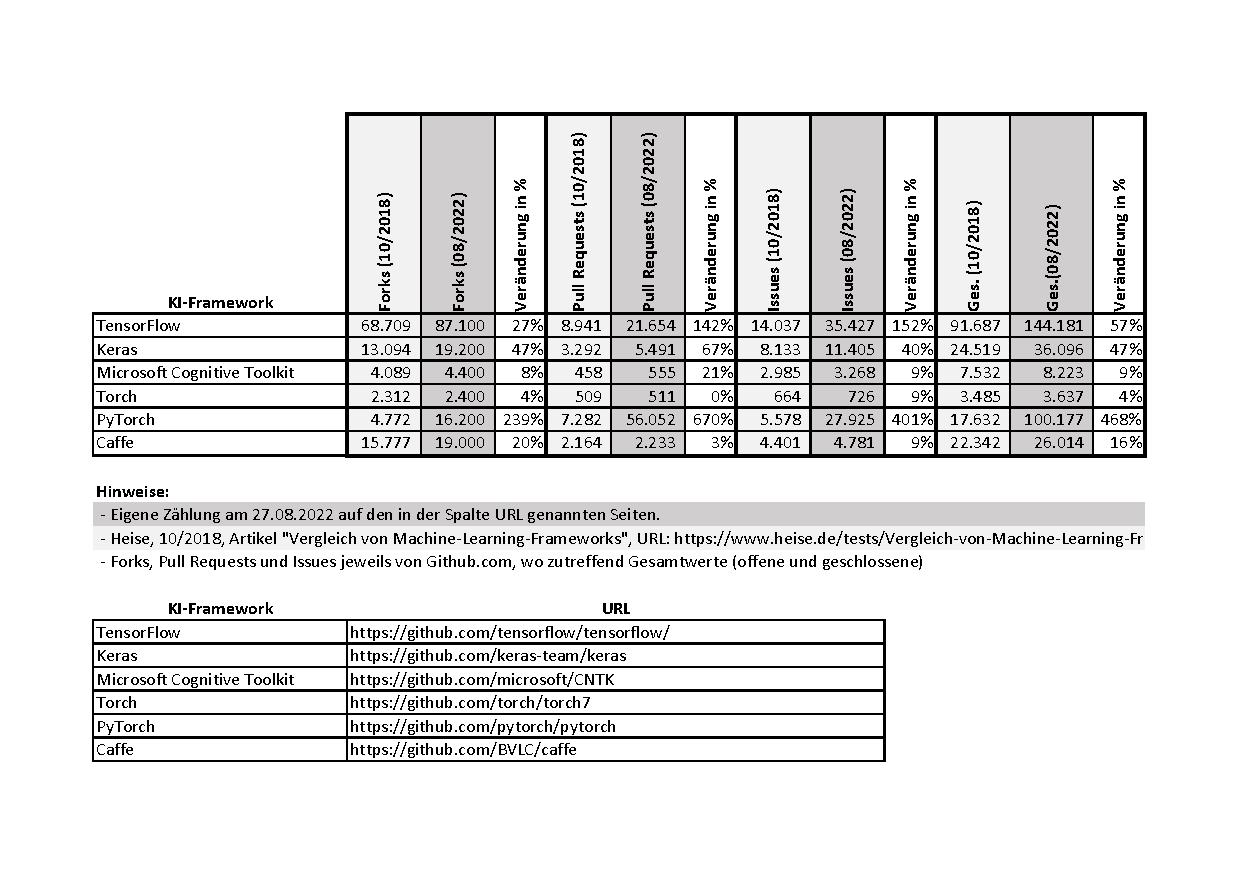
\includegraphics[width=0.98\textwidth]{ki-framework-nutzung.pdf}
	\\
	Quelle: Eigene Darstellung
\end{figure}


%Doch neben den dort auch beschriebenen technischen Hürden, wie allein dem Netzausbau, gibt es für Entwickler beim Einsatz von KI-Frameworks andere, ganz praktische Hürden. Denn wie eingangs beschrieben, gibt es verschiedenste Frameworks, in unterscheidlichsten Versionen.


\subsection{Django Web-Framework}

Django ist ein quelloffenes und frei verfügbares Web-Framework, dass nach eigenen Angaben schnell, vollständig, sicher, skalierbar und vielseitig ist \parencite[]{54-django-overview}. Untermauert wird diese eigene Behauptung von Django durch bekannte Anwendern und Nutzer wie z.B. Instagram, Pinterest und Delivery Hero \parencite{56-django-stackshare}. Eine Studie bestätigt Django weiter eine große Gemeinsachft an Entwicklern, eine bedeutsame Anzahl an Fragen und Antworten bei Stackoverflow und wird auch als gute Lösung für größere Projekte betrachtet \parencite{55-djnago-ghimire}. 

\begin{figure}[H]
	\caption{Logo des Web-Frameworks Django}\label{fig:django-logo}
	
\includegraphics[width=0.6\textwidth]{django-logo-negative.png}
	\\
	Quelle: Django Software Foundation, \url{https://www.djangoproject.com/community/logos/}
\end{figure}

Django lässt sich dabei einfach um Funktionen und Pakete erweitern. Der Modulare Aufbau mit Datenmodellen, Sichten und Einstiegspunkten lässt zusammen mit dem Template-System und der einfachen Abstraktion für verschiedene Datenbanken sowie einer praktischen Administrationsoberfläche lässt dabei dennoch eine schnelle Entwicklung von Webseiten zu.


% Aktuell ~1.200 / 1.300 Wörter -- Wenn am Ende noch Raum ist, hierzu mehr:

% \subsection{Dialogarten Direkt-, Dienst- und Jobverarbeitung}
% \subsection{Synchrone- und Asynchrone Verarbeitung}
% \subsection{Stand der Technik}

\newpage
\section{Praktischer Teil: Vom Skript zum Webservice}

Die Entwicklung erfolgt in verschiedenen Phasen, die aufeinander aufbauen. Erkenntnisse aus einer Phase, bedingen darauf folgende Schritte. Ein Wechsel zwischen den Bereichen und ein wiederholtes Aufgreifen einer Teils der Lösung, ist daher nicht als Zeichen von Unstrukturierheit zu verstehen, sondern als für den Prozess des hier angebwendeten, vertikalen Protoypings schlicht notwendig. 


\subsection{Vorbereitung einer KI-Anwendung}



Als Beispiel für bereitzustellende die KI-Anwendung wurde ein Chatbot gewählt. Eine Chatbotanwendung bietet sich an, da die Verarbeitung von menschlicher Sprache ein bedeutets Forschungsfeld innerhlab der \ac{KI} ist. Bereits seit Jahrzehnten wird in diesem Berich intensiv Forschung betrieben: Von Mitte der 1960er Jahre an mit z.B. ELIZA, einer Sprachverarbeitung die im wesentlichen auf Mustererkennung abzielt und seinerzeit vorallem durch den fehlenden Zugriff auf Informationen beschränkt war \parencite{20-weizenbaum1983eliza}. Bis hin zu jüngsten Entwicklungen die auch durch Schlagzeilen in der allegmeinen Presse Aufmerksamkeit erlangten: Microsofts Chatbot Tay funktionierte technisch, wurde aber bereits nach wenigen Tagen wieder abgeschaltet, da sich ihr Charkter in unerwünschte Richtungen entwicklte: Sie verbreitete Hassbotschaften und leugnete den Holocaust \parencite{14-heise-tay-abschaltung}. Noch mehr Aufmerksamkeit erlangte jüngst der Chatbot LaMDA von Google. Dies, da einer der Entickler, zu der Überzeugung gelangte, dass der Chatbot ein Bewusstsein und sogar eine Seele entwickelt habe \parencite[]{10-heise-google-chatbot}.

Für die Seminararbeit hier, wird jedoch nur eine sehr einfache Ausführung eines Chatbots herangzogen. Grundlage dafür ist ein Tutorial in dem der Autor \citeauthor[]{50-howto-cahtbot} Grundlagen über den  Aufbaus einer KI-Anwendung näher bringt \parencite{50-howto-cahtbot}. 

Speziell dieses Tutorial wurde gewählt, da es als KI-Framework PyTorch verwendet. PyTorch ist neben TensorFlow eines der aktuelle führenden KI-Frameworks (siehe auch Abbildung \ref{fig:ki-framework-nutzung}), hat jedoch für diesen Anwendungsfall den Vorteil, dass es deutlich weniger Abhängigkeiten hat und kleiner in der Grundinstallation ist. 

Zuerst wurde das gesamte Tutorial von mir durchgeführt und die KI-Anwendung lokal nachgebaut und getestet. Hier bei gab es keine nennenswerten Besonderheiten. Das vom Autor aufgebaute KI-Modell in der Datei \code{model.py} ist in diesem Fall ein künstliches, neuronales Netz mit drei Ebenen:

\begin{figure}[H]
	\caption{Programmcode: model.py aus Chatbot Tutorial}
	\label{fig:code-model-py-chatbot-tut}
\begin{lstlisting}[language=python]
import torch
import torch.nn as nn


class NeuralNet(nn.Module):
    def __init__(self, input_size, hidden_size, num_classes):
        super(NeuralNet, self).__init__()
        self.l1 = nn.Linear(input_size, hidden_size) 
        self.l2 = nn.Linear(hidden_size, hidden_size) 
        self.l3 = nn.Linear(hidden_size, num_classes)
        self.relu = nn.ReLU()
    
    def forward(self, x):
        out = self.l1(x)
        out = self.relu(out)
        out = self.l2(out)
        out = self.relu(out)
        out = self.l3(out)
        # no activation and no softmax at the end
        return out
\end{lstlisting}
\end{figure}

Man erkennt hier in Zeile 14 die sichtbare Eingabeebene, folgend eine verborgene Ebene Zeiel 16 sowie Ausgabeebene in Zeile 18. Da hier eine verborgene Ebene verwendet wird, spricht man von einem \enquote{Deep Learning}-Modell. Es handelt sich bei dieser \acl{KI} um ein künstliches neuronales Netz (KNN), das mit maschinellen Lernen (ML) ein mehrschichtiges bzw. tiefes Lernen (Deep Learning) durchführt. Mehr und tiefer soll in dieser Seminararbeit jedoch nicht darauf eingegangen werden, da es den Rahmen der Seminararbeit sprengen würde und nicht zum Thema selbst gehört. Deutlich wird aber, dass schon mit einer einfachen KI-Anwendung, also hier dem Einsatz des KI-Frameworks PyTorch, direkt wesentliche und grundlegnde Anwendungsfälle und mögliche Anforderungen abgedeckt werden können. Deutlich komplexere Modelle sind hier nun also nur noch eine Frage der tatsächlichen Umsetzung und eine Umsetzung scheitert hier nicht mehr an einer fehlenden IT-Infrastruktur.

Mit Abschluss des Tutorials umfasst die Anwendung nicht nur die Datei \code{model.py}, sondern auch eine \code{train.py} die er erlaubt, dass KI-Modell anhand der Eingabedaten in der Datei \code{intents.json} zu trainieren. Die Eingabedaten sind dabei wie folgt aufgebaut:


\begin{figure}[H] \caption{Auszug der Eingabedatei für das KI-Modell \enquote{intents.json}}
\label{fig:code-intents.json} \begin{lstlisting}[language=json]
{
  "intents": [
    {
    "tag"      : "Begrüßung",
    "patterns" : ["Hi", "Hallo", "Guten Tag"],
    "responses": ["Hallo auch!", "Schön dich zu sehen!", "Willkommen!"]
    },
    {
    "tag"      : "Verabschiedung",
    "patterns" : ["Tschüss", "Bis bald", "Bye"],
    "responses": [
       "Danke für das Gespräch -- Tschüss!",
       "Pass auf das die Tür zu geht. Nodda."
    ]
    }
    (...)
  ]
}
\end{lstlisting} \end{figure}

An der Struktur dieser Daten kann die Funktionsweise nachvollzogen werden: Die KI-Anwendung überprüft Eingaben und versucht diese Anhand der erlernten Muster (Zeilen 5 und 10) einem Thema (Zeilen 4 und 9) zuzuordnen. Gelingt dies mit einer bestimmten Sicherheit, werden Antworten entsprechend dem Thema (Zeilen 6 und 11-13) zurückgegeben.

Der Vollständigkeit halber verweise ich noch kurz auf den Teil der KI-Anwendung die die in dieser Eingabedatei vorhandene, natürliche Sprache verarbeitet. Bevor diese Daten für das Trainung und die Verwendung im Gespräch mit dem Chatbot verwendet werden können, müssen die mittels Algorithmen der Verarbeitung natürlicher Sprache (Natural Language Processing, NLP) für die KI aufbereitet werden. Dazu weden die Sprachdaten tokenisiert, also die Eingabe in Sätze und die Sätze in Wörter aufgeteilt. In diesem Tutorial mithilfe des Paketes \enquote{nltk} (Natural Language Toolkit).

In einem nächsten Schritt werden diese Wörter dann auf Ihren Wortstamm zurückgeführt. Dies war eine der ersten Stellen an denen ich das Ergebnis des Tutorials angepasst habe. Ich habe ein entsprechendes Paket für die Verarbeitung deutscher Sprache gesucht und mit \enquote{HanTa} gefunden \parencite[]{57-wartena2019probabilistic}. Dieser Programmablauf erfolgt nicht nur beim Trainung des KI-Modells, sondern auch beim Gespräch mit Chatbot über die \code{chat.py}.

Weitere Anpassungen durch mich in dieser allerersten Entwicklungsstufe der KI-Anwendung direkt nach Abschluss des Tutorials waren das Hinzufügen einer Log-Funktion die alle Eingaben und Antworten in Log-Dateien (hier als CSV) abspeichert. Ebenso erzeuge ich für jedes geführte Gespräch einen eindeutigen Identifikator (hier als \ac{UUID}), der es erlaubt geführte Gespräche in den Log-Dateien anhand der \ac{UUID} vollständig nachzuvollziehen. 

Alle Einstellungen und Parameter der KI-Anwendung habe ich in der Datei \code{config.py} zusammengefasst. Abschließend habe ich die für das Starten der KI-Anwendung notwendigen Abhängigkeiten und Pakete für die Verwendung mit dem Python Tool \enquote{Pipenv} in der Datei \enquote{Pipfile} zusammengefasst. 

Den gesammten ersten Entwicklungsstand, wie er bis hier beschrieben wurde, habe ich in den Anlagen zur Seminararbeit sowie auf Github.com im Unterorder \code{10-example-ai-app} dokumentiert. Die KI-Anwendung in diesem Entwicklungsstand kann ausgeführt und getestet werden indem der Ordner  \code{10-example-ai-app} mit einem Terminal betreten wird und unten stehende Befehle ausgeführt werden:


\begin{lstlisting}[language=bash]
pipenv install
pipenv run python train.py
pipenv run python chat.py
\end{lstlisting}

Vorraussetzung dafür ist ein installierter Python-Interpreter ab Version 3.9 und das Python-Tool \enquote{Pipenv}.



Für die Einbindung dieser KI-Anwendung, muss diese nun aber in einer Form vorliegen, die es erlaubt das Programm oder Programmteile an anderen Stellen einzubinden oder Teile davon aufzurufen. Die bisher vorliegende Datei- bzw. Skriptsammlung ist dazu so nicht nutzbar. Die KI-Anwendung muss daher umgebaut werden zu einem Python Modul. Ein Python Modul zeichnet sich dadurch aus, dass die notwendigen Dateien incl. einer \code{__init.py__}-Datei in einem entsprechenden Dateiordner liegen. Der Aufruf kann dann aus anderen Python Skripten mittels \code{import \textbf{NameDesModulOrdners}} aufgerufen werden. Programmfunktionen aus dem Moduls können dann mit \code{NameDesModulOrdners.\textbf{FunktionsName}} aufgerufen und gestartet werden.

Ich habe die notwendigen Anpassungen an der KI-Anwendung vorgenommen, alle Inhalte in einer Datei  zusammengetragen, gesamte Logik in passende Funktionen verpackt und aufrufbar über eine \code{main()}-Funktion gemacht. 

Als weitere Möglichkeit zum Aufruf der KI-Anwendung wurde das Modul \code{argparse} in das Modul eingebunden. Damit ist der Aufruf von Programmteilen direkt über die Konsole möglich. Das Modul \code{argparse} stellt dabei Funktionen zur Verfügung die an die Anwendung übergebene Parameter auf der Konsole parst, also Verarbeitet. Außerdem werden automatisiert, nützliche Hilfetexte für die Kommandozeile erzeugt.

Hier im Detail ein Auszug aus der Datei \code{__init.py__} des Moduls \code{chatbot}:
\begin{figure}[H]
	\caption{Programmcode: Main()-Funktion aus KI-Anwendung}
	\label{fig:code-main-func}
\begin{lstlisting}[language=python]
def main():
  parser = ArgumentParser(description='Allows the use of a chatbot with PyTorch.')

  parser.add_argument('-u', '--newuuid',  action='store_true',
            help='Get a new, unique id for a conversation.')

  parser.add_argument('-t', '--train',  action='store_true',
            help='Trains the NN model based on current data.')

  parser.add_argument('-c', '--chat',  action='store_true',
            help='Chat with the chatbot.')

  parser.add_argument('-i', '--textinput',  type=str,
            help='Give an text input to the chatbot and recive a answer. \
              Provide a UUID for the conversation with -cu or --conversationuuid \
                followed by the UUID.')

  parser.add_argument('-cu', '--conversationuuid',  type=str,
            help='Needed when using -i, --textinput. Provide a UUID to a conversation.')

  args = parser.parse_args()

  
  if vars(args)['newuuid']:
    print(str(get_new_uuid()))
    quit()

  if vars(args)['train']:
    train()
    quit()  

  if vars(args)['chat']:
    chat()
    quit()
    
  # check for complete input for a 'singlechat' call
  complete_text_input = 0
  if vars(args)['textinput']:
    complete_text_input += 1 
  if vars(args)['conversationuuid']:     
    complete_text_input += 1 

  if complete_text_input == 1:
    parser.error("Too few arguments: -cu/--conversationuuid and -i/--textinput are both needed.")
  
  if complete_text_input == 2:
    print(str(singlechat(str(args.conversationuuid), str(args.textinput))))
    quit()

  parser.print_help()


if __name__ == '__main__':
  main()
\end{lstlisting}
\end{figure}

Anhand des strukturierten Aufbaus kann man die Programmlogik und die wesentlichen Aufrufe, gut ablesen. Wird das Modul aufgerufen, springt Pyhton in die \code{main()}-Funktion (Zeilen 53 und 54). In dieser Funktion dann, wird zuerst das Modul \code{ArgumentParser} initialisiert (Zeile 2) und dann die möglichen Aufrufe über Konsolenparameter konfiguriert (Zeilen 4 bis 19). In Zeile 20 werden tatsächlich beim Programmaufruf mitgegebenen Parameter verarbeitet (geparst). Entsprechend der mitgegebenen Parameter werden dann in den Zeilen 24 bis 48 die jeweiligen je nach Programmfunktionen gestartet und das Skript beendet. Fand keine Auswahl statt, wird durch Zeile 50 das hier zu sehende Hilfemenü auf der Konsole ausgegeben:

\begin{figure}[H]
	\caption{Hilfemenü der KI-Anwendung bei Konsolenaufruf}
	\label{fig:code-help-para}
\begin{lstlisting}[language=bash]
pipenv run python -m chatbot       
usage: __main__.py [-h] [-u] [-t] [-c] [-i TEXTINPUT] [-cu CONVERSATIONUUID]

Allows the use of a chatbot with PyTorch.

options:
  -h, --help            show this help message and exit
  -u, --newuuid         Get a new, unique id for a conversation.
  -t, --train           Trains the NN model based on current data.
  -c, --chat            Chat with the chatbot.
  -i TEXTINPUT, --textinput TEXTINPUT
                        Give an text input to the chatbot and recive a answer. Provide a UUID for the conversation with  
                        -cu or --conversationuuid followed by the UUID.
  -cu CONVERSATIONUUID, --conversationuuid CONVERSATIONUUID
                        Needed when using -i, --textinput. Provide a UUID to a conversation.
\end{lstlisting} \end{figure}

Neben dem Umbau zur Python Modul und der Einbindung der Konsolenparameter, wurde noch das Logging weiter verfeinert und vervollständigt. Dieser Entwicklungsstand findet sich im Unterorder \code{20-prepared-ai-app}. Der Inhalt ist ebensfalls wieder in Anlage zu dieser Seminararbeit sowie auch auf Github.com zu finden. Der Aufruf kann wieder über die Konsole mit folgenden Befehlen erfolgen: 

\begin{lstlisting}[language=bash]
pipenv install
pipenv run python -m chatbot -t
pipenv run python -m chatbot
\end{lstlisting}

Dieser Aufruf führt dann dem oben sichtbaren Hilfemenü. Mit dem Befehl \code{pipenv run python -m chatbot -c} kann ein Chat auf der Konsole im direkten Dialog gestartet werden. 

Die Vorbereitung der KI-Anwendung, des Chatbots, kann damit an dieser Stelle abgeschlossen werden. Die Einbindung in ein anderes Pyhton Skript und auch der Aufruf über die Konsole sind möglich.
	


\subsection{Einrichtung Django Grundinstallation}

Die Bereitstellung des Webservices als REST API soll über Django erfolgen. Daher wird zuerst eine Grundinstallation von Django vorgenommen. Eine fertige Django Grundinstallation sowie die Dokumentation über die Installation findet sich in den Anlagen zur Seminararbeit und auf Github.com im Ordner \code{30-django-base-install} in der Datei \code{README.md}.

Bei dieser Installation wurden alle notwendigen Pakete und Abhängigkeiten mit berücksichtigt, die für die Einbindung der zuvor vorbereiteten KI-Anwendung notwendig waren. Auch einige weitere Pakete und Funktionen wurden vorrausschauend bereits mit installiert. Neben zwingend für die Umsetzung notwendigen Paketen wie dem \enquote{Django Toolkit für REST API}, dem \enquote{Django REST framework}, wurden voralem Pakete installiert die Funktionen bereitstellen, die den Zugriff auf die API erleichtern. 


\begin{figure}[H]
	\caption{Dateiinhalt der \enquote{Pipfile} für die Django Grundinstallation}
	\label{fig:code-nn-basis}
\begin{lstlisting}[language=python]
[[source]]
url = "https://pypi.org/simple"
verify_ssl = true
name = "pypi"

[packages]

Django = "==4.1" # Django itself 
djangorestframework = "==3.13.1" # Django toolkit for rest api
drf-yasg = "==1.21.3" # Swagger for Django / OpenAPI 2.0 
django-cors-headers = "==3.13.0" # for cross site access from a frontend
daphne = "==3.0.2" # to serve django 
whitenoise = "==6.2.0" # to serve static files
tzdata = "==2022.2" # to fix dependency error on some systems

# for the chatbot module
numpy = "==1.23.2" 
nltk = "==3.7"
HanTa = "==0.2.0" # 0.2.1 seems broken, fallback to 0.2.0
torch = "==1.12.1"

[dev-packages]

[requires]
python_version = "3"
\end{lstlisting}
\end{figure}

Über das Paket \code{drf-yasg} bzw. \enquote{Yet another Swagger generator} z.B. wird vollautomatisch eine Webseite generiert (Swagger), die der OpenAPI 2.0 Spezifikationen entspricht und Dritten damit eine vollständige Dokumentation der API bereitstellt und die Verwendung der API damit ermöglicht. 

\begin{figure}[H]
	\caption{Bildschirmfoto von lokal laufender Swagger Instanz}\label{fig:local-swagger}
	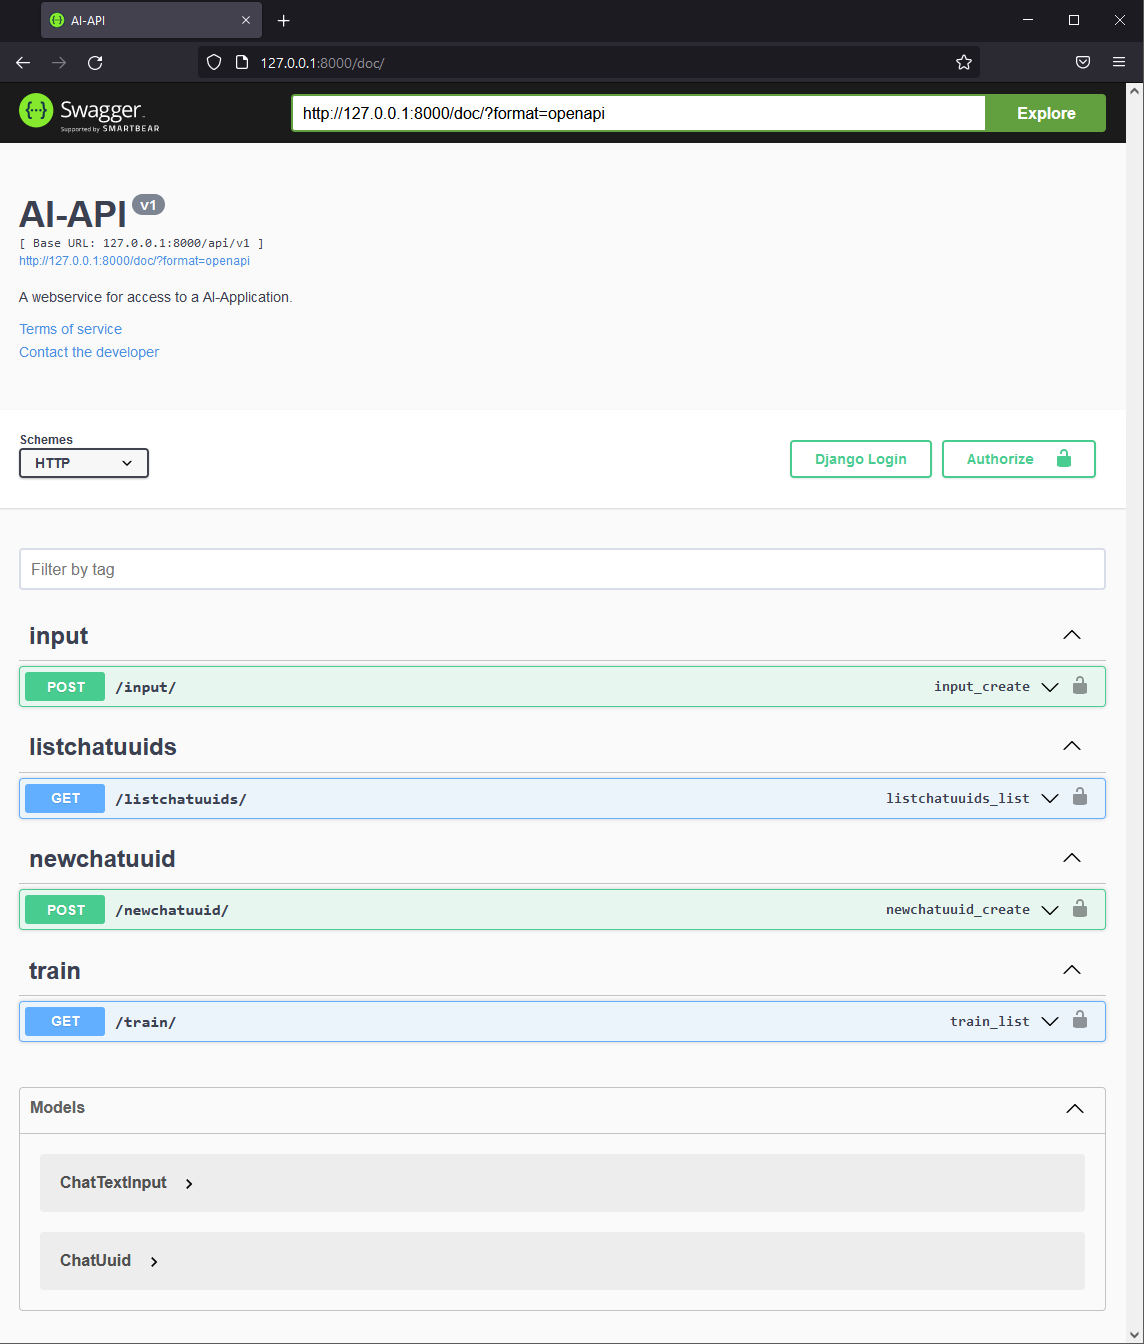
\includegraphics[width=0.60\textwidth]{swagger.png}
	\\
	Quelle: Eigenes Bildschirmfoto
\end{figure}


Der Installations- und Einrichtungsporzess ist bei Django gut zu dokumentiern. Die Schritte sind kleinteilig und führen, in der korrekten Abfolge ausgeführt, regelmäßig zum gleichen Ergebnis. Für diese Grundinstallation sind 14 Schritte erforderlich, die in einem Zeitraum von etwa 30 Minuten von einer  Person mit IT-Kenntnissen gut abgearbeitet werden können. Es müssen z.B. verschiedene Konsolenbefehle, wie z.B. \code{pipenv run python manage.py createsuperuser} für die Anlage eines Administratoraccounts oder \code{pipenv run python -m chatbot -t} zum initialen Training des KI-Modells, eingegeben werden. Auch müssen verschiedene Dateien angelegt oder bestehenden Datein Inhalte an der korrekten Stelle hinzugefügt werden. Dazu ein Auszug aus der Anleitung: 

\begin{figure}[H]
	\caption{Auszug der \enquote{README.md}-Datei: Zeilenweise Konfiguration}
	\label{fig:code-django-readme}
\begin{lstlisting}[language=python]
# Pay attention to the order:
MIDDLEWARE = [
    'corsheaders.middleware.CorsMiddleware', # add cors as the first line
    ...
    'django.middleware.security.SecurityMiddleware', # look out for this line and insert whitenoise below
    'whitenoise.middleware.WhiteNoiseMiddleware', # for static files
    ...
\end{lstlisting}
\end{figure}

Neben diesen einfacherern Schritten, war es aber auch notwendig die KI-Anwendung selbst einzubinden. Dazu wird während des Installationprozesses die KI-Anwendung aus dem Ordner \code{20-prepared-ai-app} in den Ordner der Django Grundinstallation kopiert. Damit können Funktionen der KI-Anwendung als Modul an jeder Stelle von Django importiert und aufgerufen werden. 

Dann folgend müssen für die Funktionen der KI-Anwendung entsprechende Programmierungen in Django erstellt werden: Das Datenmodell muss abgebildet werden, die Sichten auf die Daten müssen ertellt werden und die entsprechenden Einstiegspunkte konfiguriert werden. Innerhalb von Django finden sich diese Programmierungen bzw. Konfigurationen in den Dateien \code{models.py}, \code{views.py} und \code{urls.py} wieder. Je nach Organisation finden sich diese Dateien an unterscheidlichen Stellen von Django wieder. Auch lassen sich die Inhalte auf verschiedene Hirachien aufteilen und damit nach Programmteil getrennt hinterlegen. Das kann die Organisation von Anwendungen deutlich erleichtern.

In den in Django agelegten Datenmodellen erkennt mal z.B. schnell, dass diese vom Aufbau im wesentlichen den bisherigen Log-Dateien entsprechen. Folgend sind die beiden Klassen zu den Datenmodellen zu sehen. Wie man erkennt, können diese auch mit Informationen angereichert werden, die im Webservice wichtige Hinweise zur korrekten Nutzung geben:

\begin{figure}[H]
	\caption{Auszug der \enquote{models.py}-Datei: Das Django Datenmodell}
	\label{fig:code-django-data-modell}
\begin{lstlisting}[language=python]
class ChatUuid(models.Model):
    chatuuid = models.UUIDField(unique=True, default=uuid.uuid4,
                                editable=False, help_text="The UUID for a Chatbot conversation.")
    created = models.DateTimeField(auto_now_add=True)
    agreed = models.TextField(
        blank=True, help_text="If user agreed to the service terms (http://...), send 'Einverstanden'.")

    def __str__(self):
        return str(self.chatuuid)

class ChatDialogue(models.Model):
    chatuuid = models.UUIDField(blank=False)
    created_at = models.DateTimeField(auto_now_add=True)
    updated_at = models.DateTimeField(auto_now=True)
    input = models.TextField(blank=False)
    probability = models.FloatField(blank=True)
    understood = models.BooleanField(blank=True)
    output = models.TextField(blank=True)

    def __str__(self):
        return str(self.input)
\end{lstlisting}
\end{figure}

So kann man durch die Angaben im Attribut \code{help_text='...'} in den Zeilen 3 und 6 der Abbildung \ref{fig:code-django-data-modell} hinterlegen, was für Nutzer der API relevant ist. Hier wird z.B. der Klasse \code{ChatUuid} die Information mitgegeben, dass es sich dabei um eine \ac{UUID} für ein Gespräch mit dem Chatbot handelt. Eine ChatUuid aber, wird nur vergeben, so das Einverständnis zu den Nutzungsbedinungen erteilt wurde. Hier indem der Parameter \code{agreed} mit dem Inhalt \enquote{Einverstanden} übergeben wurde. Eine entsprechende Fehlermeldung wurde über einen Inhalt in der Datei \code{views.py} programmiert: 

\begin{figure}[H]
	\caption{Auszug der \enquote{views.py}-Datei: Die Django Sichten}
	\label{fig:code-django-views}
\begin{lstlisting}[language=python]
class ChatUuidNewAPIView(CreateAPIView):
    model = ChatUuid
    serializer_class = ChatUuidSerializer
    queryset = ChatUuid.objects.all()

    def post(self, request, *args, **kwargs):
        request.data["chatuuid"] = get_new_uuid()

        if request.data["agreed"] != "Einverstanden":
            return Response(data="If 'agreed' is not 'Einverstanden' you can not use the services.",
                            status=status.HTTP_400_BAD_REQUEST)

        return self.create(request, *args, **kwargs)
\end{lstlisting}
\end{figure}

In Abbildung \ref{fig:code-django-views} findet man ein Klasse des Typs \code{CreateAPIView}. Diese stellt über des \enquote{Djangao Rest framework} einen Endpunkt für POST Anfragen bereit. In der Zeile 6 sieht man entsprechend ein die Methode \code{def post(...):}. Die Programmlogik für die Fehlermeldung findet sich in der Zeilen 9: Hier wird überprüft ob der bereits bekannte Parameter \code{agreed} mit dem Inhalt \enquote{Einverstanden} befüllt ist. Ist das nicht der Fall, wird über Zeile 10 eine Rückgabe mit Fehlermeldung und HTTP-Statuscode 400 (keine Verarbeitung aufgrund clientseitigem Fehler) zurückgegeben.

Nach dieser Systematik wurden für alle Funktionen der KI-Anwendung entsprechend Sichten und Einstiegspunkte programmiert, die der Installationsanleitung \code{30-django-base-install\\README.md} in den Anlagen und auf Github.com entnommen werden kann. Auch finden sich natürlich alle Programmierungen und Konfigurationen in dem Ordner zur Django Grundinstallation selbst (\code{30-django-base-install}). 

Den vollständigen Ordnerinhalt zeigt die folgende Abbildung: 

\begin{figure}[H]
	\caption{Ordnerinhalt Django Grundinstallation}\label{fig:img-django-base-install}
	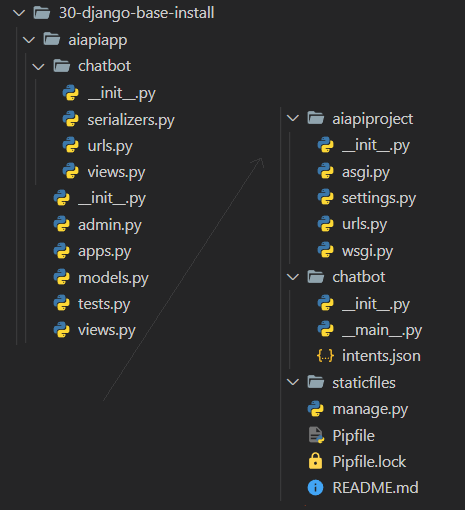
\includegraphics[width=0.5\textwidth]{django-folder.png}
	\\
	Quelle: Eigenes Bildschirmfoto
\end{figure}

Für die API wurden insgesamt vier Endpunkte, also die Zugriffspunkte auf die KI-Anwendung, erstellt. Zwei der Endpunkte, \code{input} und \code{newchatuuid}, sind dabei für das Gespräch mit dem Chatbot notwendig. Mittels einer POST HTTP-Anfrage an \code{/api/v1/chatbot/input} können schon mit den beiden Pflichtparametern \code{input} und \code{chatuuid} Eingaben an die KI-Anwendung übergeben werden. Der Chatbot verarbeitet diese dann über den Modulaufruf aus einer Django Sicht bzw. View heraus, und gibt die Antwort im Feld \code{output}, zusammen mit eineigen anderen Feldern wie z.B. der Wahrscheinlichkeit des Verständnisses, im direkten Dialog als Antwort auf die Anfrage selbst, mit einem HTTP-Statuscode 200 (erfolgreich) zurück wie die folgende Abbildung zeigt:

\begin{figure}[H]
	\caption{Antwort des Webservices auf Chatbot-Eingabe}\label{fig:img-cb-200-input}
	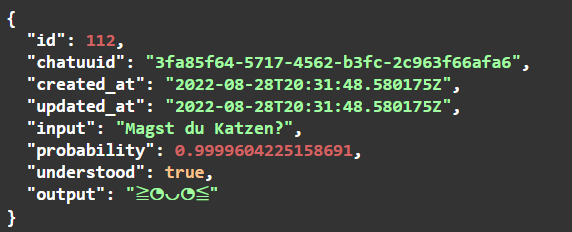
\includegraphics[width=0.7\textwidth]{status200-input.png}
	\\
	Quelle: Eigenes Bildschirmfoto
\end{figure}


Einen weiteren Endpunkt gibt es zum Trainung des KI-Modells, den \code{/api/v1/chatbot/train}. Dieser Endpunk ist für die Verwendung mit einer GET Methode angelegt. Der Aufruf jedoch, wird nur erlaubt wenn über eine HTTP Basis Authentifizierung ein Benutzername und das entsprechende Passwort eines Administratorkontos der Anfrage mitegegeben wird. Bei fehlenden Authentifizierungsdaten erfolgt die Antwort mit HTTP-Statuscode 403 (verboten) und der Fehlermeldung \code{ \{ "detail": "Authentication credentials were not provided." \}}. Werden falsche Angaben gemacht, eroflgt die Antwort mit geleichem Statuscode, jedoch der Fehlermeldung \code{ \{ "detail": "Invalid username/password." \}}. Diese Fehlermeldungen werden dabei von Django bzw. dem \enquote{Django Rest framework} automatisch erzeugt und übermittelt. Die einzige Einstellung dazu erfolgte in den Sichten, der Datei \code{views.py}, in Zeile 2 durch eine Angabe im Parameter \code{permission_classes}:

\begin{figure}[H]
	\caption{Auszug der \enquote{views.py}-Datei: Berechtigungen einer Klasse}
	\label{fig:code-django-views-admin-only}
\begin{lstlisting}[language=python]
class ChatTrainAPIView(views.APIView):
    permission_classes = [permissions.IsAdminUser]

    def get(self, request, format=None):
        """
        Returns the console output from the training process.
        Only Admin Users can start the training.
        """
        trainoutput = train()
        
        return Response(data=str(trainoutput), status=status.HTTP_200_OK)
\end{lstlisting}
\end{figure}




% \subsection{Erweiterungen für API}
% \subsection{Pyhton Module und Pakete}
% \subsection{Aufruf als Subprozess}
% \subsection{Zugriff}
% \subsubsection{Konsolenbasiert mit Zeitmessung}
\subsection{Zugriff mit Vue.js und Axios auf Web-Frontend}

\section{Fazit und Reflexion}




%-----------------------------------
% Apendix / Anhang
%-----------------------------------
%\newpage
%\section*{\AppendixName} %Überschrift "Anhang", ohne Nummerierung
%\addcontentsline{toc}{section}{\AppendixName} %Den Anhang ohne Nummer zum Inhaltsverzeichnis hinzufügen

%\begin{appendices}
% Nachfolgende Änderungen erfolgten aufgrund von Issue 163
%\makeatletter
%\renewcommand\@seccntformat[1]{\csname the#1\endcsname:\quad}
%\makeatother
%\addtocontents{toc}{\protect\setcounter{tocdepth}{0}} %
%	\renewcommand{\thesection}{\AppendixName\ \arabic{section}}
	%\renewcommand\thesubsection{\AppendixName\ \arabic{section}.\arabic{subsection}}
	% haenno-apa6-slim: Start
	% \input{kapitel/anhang/anhang}

	%\section{Beispielanhang}\label{Beispielanhang}
	%Dieser Abschnitt dient nur dazu zu demonstrieren, wie ein Anhang aufgebaut seien kann.
	%\subsection{Weitere Gliederungsebene}
	%Auch eine zweite Gliederungsebene ist möglich.

	% haenno-apa6-slim: End
%\end{appendices}
%\addtocontents{toc}{\protect\setcounter{tocdepth}{2}}


%-----------------------------------
% Literaturverzeichnis
%-----------------------------------
\newpage

% Die folgende Zeile trägt ALLE Werke aus literatur.bib in das
% Literaturverzeichnis ein, egal ob sie zietiert wurden oder nicht.
% Der Befehl ist also nur zum Test der Skripte sinnvoll und muss bei echten
% Arbeiten entfernt werden.
%\nocite{*}

%\addcontentsline{toc}{section}{Literatur}

% Die folgenden beiden Befehle würden ab dem Literaturverzeichnis wieder eine
% römische Seitennummerierung nutzen.
% Das ist nach dem Leitfaden nicht zu tun. Dort steht nur dass 'sämtliche
% Verzeichnisse VOR dem Textteil' römisch zu nummerieren sind. (vgl. S. 3)
%\pagenumbering{Roman} %Zähler wieder römisch ausgeben
%\setcounter{page}{4}  %Zähler manuell hochsetzen

% Ausgabe des Literaturverzeichnisses

% haenno-apa6-slim: Start

% Im Literaturverzeichnis "und" wieder durch "&" ersetzen	
\DeclareDelimFormat*{finalnamedelim}{\addspace\&\space}

% Punkt hinter und vor der Jahreszahl entfernen	- Wichtig für Quell-Arten wie misc und online -- Sonst ein überflüssiger Punkt im LitVerz.
	\renewbibmacro*{author}{%
	\printtext{%
	\ifnameundef{author}
	{\usebibmacro{labeltitle}}
	{\printnames[apaauthor][-\value{listtotal}]{author}%
	\setunit*{\addspace}%
	\printfield{nameaddon}%
	\ifnameundef{with}
	{}
	{\setunit{}\addspace\mkbibparens{\printtext{\bibstring{with}\addspace}%
	\printnames[apaauthor][-\value{listtotal}]{with}}
	\setunit*{\addspace}}}%
	% \newunit\newblock%
	\usebibmacro{labelyear+extradate}}}

% haenno-apa6-slim: End

% Keine Trennung der Werke im Literaturverzeichnis nach ihrer Art
% (Online/nicht-Online)
%\begin{RaggedRight}
%\printbibliography
%\end{RaggedRight}

% Alternative Darstellung, die laut Leitfaden genutzt werden sollte.
% Dazu die Zeilen auskommentieren und folgenden code verwenden:

% Literaturverzeichnis getrennt nach Nicht-Online-Werken und Online-Werken
% (Internetquellen).
% Die Option nottype=online nimmt alles, was kein Online-Werk ist.
% Die Option heading=bibintoc sorgt dafür, dass das Literaturverzeichnis im
% Inhaltsverzeichnis steht.
% Es ist übrigens auch möglich mehrere type- bzw. nottype-Optionen anzugeben, um
% noch weitere Arten von Zusammenfassungen eines Literaturverzeichnisse zu
% erzeugen.
% Beispiel: [type=book,type=article]
\printbibliography[nottype=online,heading=bibintoc,title={\langde{Literaturverzeichnis}\langen{Bibliography}}]

% neue Seite für Internetquellen-Verzeichnis
\newpage

% Laut Leitfaden 2018, S. 14, Fussnote 44 stehen die Internetquellen NICHT im
% Inhaltsverzeichnis, sondern gehören zum Literaturverzeichnis.
% Die Option heading=bibintoc würde die Internetquelle als eigenen Eintrag im
% Inhaltsverzeicnis anzeigen.
%\printbibliography[type=online,heading=bibintoc,title={\headingNameInternetSources}]
\printbibliography[type=online,heading=subbibliography,title={\headingNameInternetSources}]

% haenno-apa6-slim: Start
% \input{kapitel/anhang/erklaerung}
\newpage
\pagenumbering{gobble} % Keine Seitenzahlen mehr

%-----------------------------------
% Ehrenwörtliche Erklärung
%-----------------------------------
\section*{%
	\langde{Ehrenwörtliche Erklärung}
	\langen{Declaration in lieu of oath}}
\langde{Hiermit versichere ich, dass die vorliegende Arbeit von mir selbstständig und ohne unerlaubte Hilfe angefertigt worden ist, insbesondere dass ich alle Stellen, die wörtlich oder annähernd wörtlich aus Veröffentlichungen entnommen sind, durch Zitate als solche gekennzeichnet habe. Ich versichere auch, dass die von mir eingereichte schriftliche Version mit der digitalen Version übereinstimmt. Weiterhin erkläre ich, dass die Arbeit in gleicher oder ähnlicher Form noch keiner Prüfungsbehörde/Prüfungsstelle vorgelegen hat. Ich erkläre mich damit nicht einverstanden, dass die Arbeit der Öffentlichkeit zugänglich gemacht wird. Ich erkläre mich damit einverstanden, dass die Digitalversion dieser Arbeit zwecks Plagiatsprüfung auf die Server externer Anbieter hochgeladen werden darf. Die Plagiatsprüfung stellt keine Zurverfügungstellung für die Öffentlichkeit dar.}
\langen{I hereby declare that I produced the submitted paper with no assistance from any other party and without the use of any unauthorized aids and, in particular, that I have marked as quotations all passages which are reproduced verbatim or near-verbatim from publications. Also, I declare that the submitted print version of this thesis is identical with its digital version. Further, I declare that this thesis has never been submitted before to any examination board in either its present form or in any other similar version. I herewith \textcolor{red}{agree/disagree} that this thesis may be published. I herewith consent that this thesis may be uploaded to the server of external contractors for the purpose of submitting it to the contractors’ plagiarism detection systems. Uploading this thesis for the purpose of submitting it to plagiarism detection systems is not a form of publication.}


\par\medskip
\par\medskip

\vspace{5cm}

\begin{table}[H]
	\centering
	\begin{tabular*}{\textwidth}{c @{\extracolsep{\fill}} ccccc}
		\myOrt, \today
		&
		% Hinterlege deine eingescannte Unterschrift im Verzeichnis /abbildungen und nenne sie unterschrift.png
		% Bilder mit transparentem Hintergrund können teils zu Problemen führen
		
\includegraphics[width=0.35\textwidth]{unterschrift_henning.png}\vspace*{-0.35cm}
		\\
		\rule[0.5ex]{12em}{0.55pt} & \rule[0.5ex]{12em}{0.55pt} \\
		\langde{(Ort, Datum)}\langen{(Location, Date)} & \langde{(Eigenhändige Unterschrift)}\langen{(handwritten signature)}
		\\
	\end{tabular*} \\
\end{table}

% haenno-apa6-slim: End
\end{document}


